\documentclass{article} % For LaTeX2e
\usepackage[T1]{fontenc}
\usepackage{iclr2027_conference,times}

% Optional math commands from https://github.com/goodfeli/dlbook_notation.
\input{math_commands.tex}

\usepackage{hyperref}
\usepackage{url}
\usepackage{booktabs}
\usepackage{array}
\usepackage{siunitx}
\sisetup{detect-weight=true, retain-explicit-plus=true}
\usepackage{graphicx}
\usepackage{amsmath}
\usepackage{amssymb}
\usepackage{amsthm}
\newtheorem{proposition}{Proposition}
\newtheorem{lemma}{Lemma}
\usepackage{xcolor}

% ---------------------------------------------------------------------------
% Recurring names: methods, models, benchmarks, harnesses, and headline
% numbers are defined once here and used everywhere via macros, so a renamed
% method or an updated measurement is a one-line change.
% Call with trailing {} in text (e.g. \swev{} accuracy) to protect spacing.
% ---------------------------------------------------------------------------
% method & components
\newcommand{\HP}{\textsc{Harness Protocol}}
\newcommand{\method}{\textsc{Hint}}
\newcommand{\chr}{\textsc{Chr}}
\newcommand{\cham}{\textsc{Chameleon}}
% models
\newcommand{\basemodel}{Qwen3.6-35B-A3B}
\newcommand{\oldmodel}{Qwen3-30B-A3B-Instruct-2507}   % base model of the earlier run (Appendix C)
% benchmarks
\newcommand{\swev}{SWE-bench Verified}
\newcommand{\swem}{SWE-bench Multilingual}
% harnesses
\newcommand{\claudecode}{Claude Code}
\newcommand{\opencode}{OpenCode}
\newcommand{\codexcli}{Codex CLI}
\newcommand{\openhands}{OpenHands SDK}   % the harness the code calls r2e-gym is an internal OpenHands SDK build; the paper describes OpenHands SDK by its current tool surface (terminal / file_editor / task_tracker / finish)
% baseline
\newcommand{\control}{step-matched control}
% headline measurements (single source of truth)
\newcommand{\numactions}{578{,}856}       % tool calls parsed from the four harness corpora
\newcommand{\numtraj}{9{,}873}            % trajectories parsed
\newcommand{\numroundtrip}{1.87M}         % render-parse checks (578,856 actions x 3-4 sampled surfaces each)
\newcommand{\rtacc}{100.0000\%}           % round-trip consistency
\newcommand{\numsurfaces}{26{,}031}       % distinct surface configs in training (one per rendered sample)
% utilities
\newcommand{\todo}[1]{\textcolor{red}{[#1]}}

\title{HINT: Learning the Harness Protocol for\\
Interface-Invariant SWE Agents}

\author{Anonymous Authors \\
Affiliation \\
\texttt{email}
}

\newcommand{\fix}{\marginpar{FIX}}
\newcommand{\new}{\marginpar{NEW}}

%\iclrfinalcopy % Uncomment for camera-ready version, but NOT for submission.
% Top-of-page floats leave the text column short; with the style's flush bottom
% that shortfall was stretched into 60pt gaps under captions.
\raggedbottom

\begin{document}

\maketitle

\begin{abstract}
Large language model (LLM) agents now resolve real GitHub issues by exploring
a repository, editing files and running tests. Each runs inside a
\emph{harness} such as \claudecode{}, \codexcli{}, \opencode{} or
\openhands{}, the scaffold that fixes which tools the model sees, their
names, and how calls and results are formatted. These details differ across
harnesses and they matter: with model and tasks fixed, changing only the
harness moves \swev{} accuracy by up to $9.0$ points. Because training
trajectories come from one harness, fine-tuning learns the interface with the
task, and its gains largely stay there. This dependence is avoidable because
the differences are superficial: \numactions{} real tool calls from four
production harnesses all reduce to $12$ semantic actions, which we call the
\HP{}. A harness is this protocol plus a \emph{surface} of tool names,
documentation, output and turn formatting, and a trajectory rendered into any
surface parses back to the same actions (\numroundtrip{} checks, no
mismatches). \method{} (Harness-INvariant Training) parses each real
trajectory into the protocol and re-renders it under many sampled surfaces,
some with tool names replaced by meaningless identifiers, so that one
harness's data trains an agent for any harness with no new task data.
Fine-tuning \basemodel{} on \claudecode{} trajectories, \method{} matches a
step-matched control on \claudecode{} itself, leads under every unseen
production harness by up to $8.7$ points, narrows the \swem{} accuracy range across five
harnesses from $7.4$ to $1.6$ points, and is on a par with a model trained on
real trajectories from four harnesses. Harness variation is thus a nuisance
factor that training can marginalize over, not a distribution shift the agent
must absorb.
\end{abstract}

\section{Introduction}
\label{sec:intro}

Recent years have seen rapid progress in LLM agents for software engineering.
Given an issue reported against a real GitHub repository, an agent such as
\claudecode{} \citep{anthropic2025claudecode}, \codexcli{}
\citep{openai2025codex}, \opencode{} \citep{opencode2025} or \openhands{}
\citep{wang2025openhandssdk} explores the codebase,
edits files, runs tests, and returns a patch, and SWE-bench
\citep{jimenez2024swebench} has become the standard measure of how often that
patch is correct. Underneath every such agent is a language model wrapped in a
scaffold: a system prompt that documents a tool set, a protocol for emitting
calls, an executor, and a formatter that returns observations. This wrapper, the \emph{harness} (also called a scaffold), is what the model actually sees.

The four harnesses above all let an agent run shell commands and edit files,
but they disagree on nearly every detail of how: whether reading a file is a
first-class tool or a shell command, whether that tool is called \texttt{Read}
or \texttt{read} or \texttt{file\_editor} with
\texttt{command="view"}, whether output carries line numbers, and whether an
episode ends with a \texttt{finish} call or a plain reply. These are
presentational choices, and one would expect them not to matter, but they do.
Changing \emph{only} the harness for a fixed instruction-tuned model and task
set (Table~\ref{tab:e0}) moves \swev{} accuracy by up to $9.0$ points, from $58.6\%$ to $67.6\%$ for Qwen3.5-35B-A3B across five
harnesses. Training makes the dependence worse: trajectories are collected in
whichever harness the data pipeline uses, and supervised fine-tuning (SFT) on
them teaches the task \emph{and} the surface at once, so a different harness at deployment is,
from the model's perspective, a change of task (Figure~\ref{fig:overview},
left). Fine-tuning \basemodel{} on \claudecode{} trajectories raises its
\claudecode{} accuracy on \swev{} from $69.0\%$ to $78.4\%$ but moves its
\codexcli{} accuracy by less than the noise floor ($68.0\%$ before, $66.7\%$
after), widening its spread across harnesses from $3.4$ to $11.7$ points
(Section~\ref{sec:step-matched}).

\begin{figure}[t]
\begin{center}
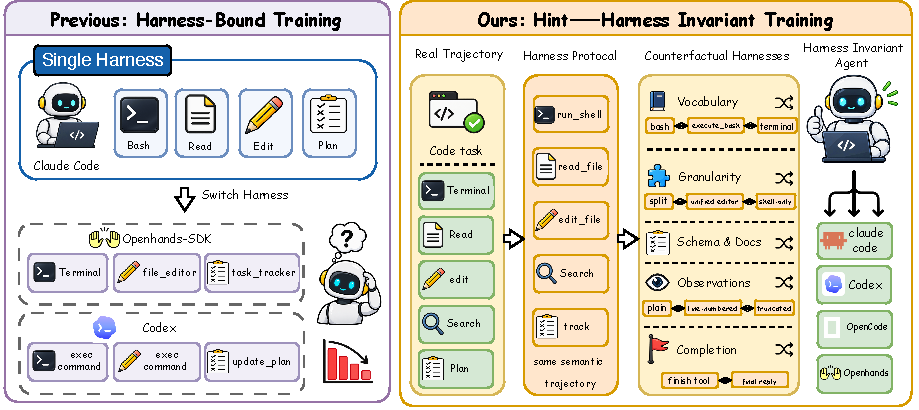
\includegraphics[width=\textwidth]{pic/intro_v1.pdf}
\end{center}
\caption{\textbf{Left:} standard agent training binds the policy to the one
harness its trajectories were collected in, and moving the model to a harness
with different tools and conventions degrades performance on the same tasks.
\textbf{Right:} \method{} parses each real trajectory down to the \HP{}, the
semantic core all harnesses share, and re-renders it into many counterfactual
harnesses whose surface axes are independently resampled, training an agent
that is invariant to the surface rather than bound to it.}
\label{fig:overview}
\end{figure}

We argue that this shift is avoidable, because the disagreement between
harnesses is superficial in a measurable sense. Normalizing \numactions{} tool
calls from the four harnesses into semantic actions, we find that a
vocabulary of $12$ covers $99.96\%$ of them (Table~\ref{tab:vocab}): the
harnesses are not doing different things, they are naming and packaging the
same things differently. We make this core explicit and call it the \HP{}. A
concrete harness is then the protocol plus a \emph{surface}, five axes that
can be set independently: tool granularity and naming, call syntax, prompt
documentation, observation formatting, and turn conventions. The abstraction
is not lossy: rendering a protocol trajectory into a surface and parsing it
back recovers the original actions, with no mismatches in \numroundtrip{}
render--parse checks over all \numactions{} actions
(Section~\ref{sec:protocol}). This is a \emph{descriptive} claim about
harnesses that already exist, not a proposal for a new standard.

Exact invertibility is what turns the protocol from an analysis tool into a
training signal. If a real trajectory can be parsed into protocol form and
re-rendered in an arbitrary surface, then a single collected episode represents an entire family of equivalent
episodes. We introduce \method{} (Harness-INvariant Training), which trains on
that family
(Figure~\ref{fig:overview}, right). Counterfactual harness rendering (\chr{})
re-renders every trajectory under freshly sampled surface configurations, and
interface anonymization replaces tool names with meaningless identifiers on a
fraction of samples, so that reading the documentation rather than recognizing
the name becomes the only reliable strategy. \method{} needs no new task data
and no architectural change.

We fine-tune \basemodel{} on \claudecode{} trajectories and evaluate under real
harnesses that training never showed as coherent wholes, against a \control{}
trained on the same trajectories in their original harness for the same number
of optimizer steps. \method{} matches the control on the source harness, is
ahead on both benchmarks under each of the three unseen production harnesses,
by up to $8.7$ points, and on \swem{} its accuracy varies by $1.6$ points
across five harnesses against the control's $7.4$
(Section~\ref{sec:step-matched}). Harness variation, in other words, is not a
property of the task that a model must absorb, but a nuisance factor that a
training pipeline can marginalize over. Our contributions are:
\begin{itemize}
\item \textbf{The \HP{}}: harness choice alone moves \swev{} by up to
  $9.0$ points for a fixed model and task set, yet \numactions{} real tool
  calls from four harnesses reduce to a $12$-action vocabulary with
  invertible surface rendering, which we formalize as the protocol
  (Sections~\ref{sec:protocol} and~\ref{sec:harness-choice}).
\item \textbf{\method{}}: training on counterfactual renderings of existing
  trajectories, with no new task data and no architecture change
  (Section~\ref{sec:method}).
\item \textbf{Experiments}: a step-matched evaluation under five harnesses
  (Section~\ref{sec:step-matched}), a comparison with real trajectories from
  four harnesses (Section~\ref{sec:real}), and analyses of test-time
  anonymization and of one surface axis at a time (Sections~\ref{sec:anon}
  and~\ref{sec:axes}).
\end{itemize}

\section{The Harness Protocol}
\label{sec:protocol}

\subsection{Semantic actions and surfaces}

Reading a file is a \texttt{Read} call in \claudecode{}, a \texttt{read} call
in \opencode{}, a \texttt{file\_editor} call with \texttt{command="view"} in
\openhands{}, and a \texttt{sed -n} or \texttt{cat} command under \codexcli{};
the protocol records all four as the same action, \texttt{read\_file}, and
treats everything else about the call as a property of the harness.

\paragraph{Semantic actions.} Let $\mathcal{A}$ be a finite vocabulary of
semantic actions, each a pair of a verb and a typed argument record. We take
$\mathcal{A}$ to be the $12$ actions of Table~\ref{tab:vocab}, obtained by
normalizing four harnesses' tool sets rather than by design; only $0.04\%$ of
the \numactions{} real calls we parsed fall outside it. A \emph{protocol
trajectory} is a sequence $\tau = \big[(c_t, a_t, o_t)\big]_{t=1}^{T}$ where
$a_t \in \mathcal{A}$ is an action, $o_t$ the semantic content of the resulting
observation with formatting removed, and $c_t$ the agent's reasoning text.

\paragraph{Harnesses as renderings.} A harness $h$ is a rendering function $R_h$
mapping a protocol trajectory to a surface trajectory: the concrete token
sequence a model consumes and produces. We use \emph{surface} and
\emph{interface} interchangeably for this rendering, and \emph{harness} for the
whole system that also executes the actions. Writing $\mathcal{H}$ for the
space of harnesses, we factor the surface into five axes,
\begin{equation}
\mathcal{H} \;=\; A_1 \times A_2 \times A_3 \times A_4 \times A_5 ,
\label{eq:axes}
\end{equation}
with $A_1$ tool granularity and naming, $A_2$ call syntax, $A_3$ system-prompt
template and tool-documentation style, $A_4$ observation formatting, and $A_5$
turn and completion conventions. A harness is a point $h \in \mathcal{H}$;
sampling a point is sampling a synthetic harness (Appendix~\ref{app:orbit}
shows one trajectory under three such points).

\begin{table}[b]
\caption{The $12$-action vocabulary recovered by normalizing four harnesses,
with its distribution over $\numactions{}$ real tool calls. \texttt{unknown} is not
part of the vocabulary; it is the residual, and its size bounds the coverage
error. Percentages are rounded independently and need not sum to $100$.}
\label{tab:vocab}
\begin{center}
\begin{small}
\begin{tabular}{lrlr}
\toprule
Action & Share & Action & Share \\
\midrule
\texttt{run\_shell}              & $71.52\%$ & \texttt{edit\_file/write}  & $0.84\%$ \\
\texttt{read\_file}              & $13.59\%$ & \texttt{web\_fetch}        & $0.39\%$ \\
\texttt{edit\_file/str\_replace} & $7.22\%$  & \texttt{web\_search}       & $0.14\%$ \\
\texttt{search}                  & $3.26\%$  & \texttt{delegate}          & $0.04\%$ \\
\texttt{submit}                  & $1.62\%$  & \texttt{edit\_file/undo}   & $0.01\%$ \\
\texttt{task\_track}             & $1.34\%$  & \texttt{edit\_file/insert} & $<0.01\%$ \\
\midrule
\multicolumn{4}{l}{\texttt{unknown} (residual, outside the vocabulary): $0.04\%$}\\
\bottomrule
\end{tabular}
\end{small}
\end{center}
\end{table}

\begin{table}[t]
\caption{Four production harnesses agree on semantics and disagree on
everything else. ``Tools'' counts the standard declared schema; granularity is
the $A_1$ setting each harness occupies, where shell only means that files are
read, searched and edited through shell commands rather than first-class tools.
Tool names are those of the releases in our parsed corpora; the releases
evaluated in Section~\ref{sec:exp} rename a few of them (Appendix~\ref{app:eval}).}
\label{tab:harnesses}
\begin{center}
\begin{small}
\begin{tabular}{lrlll}
\toprule
Harness & Tools & Granularity & Shell tool & File read \\
\midrule
\openhands{}     & $4$  & unified editor & \texttt{terminal}      & \texttt{file\_editor} \\
\opencode{}      & $11$ & split          & \texttt{bash}          & \texttt{read} \\
\codexcli{}     & $13$ & shell only     & \texttt{exec\_command} & --- (via shell) \\
\claudecode{}   & $21$ & split          & \texttt{Bash}          & \texttt{Read} \\
\bottomrule
\end{tabular}
\end{small}
\end{center}
\end{table}

Table~\ref{tab:harnesses} places the four production harnesses in this space,
and the extremes are instructive. \openhands{} exposes $4$ tools; \claudecode{} exposes $21$.
\codexcli{} declares $13$ tools but \emph{none} of them reads, edits or searches
files: $97\%$ of its calls go to a single \texttt{exec\_command} entry point,
and of those command bodies $27\%$ are file reads (\texttt{sed -n},
\texttt{cat}, \texttt{head}), $18\%$ are searches (\texttt{grep},
\texttt{find}), and $10\%$ are patch applications. More than half of \codexcli{}'s
shell traffic is, semantically, what other harnesses expose as first-class
tools. Surface variation of this magnitude over an identical semantic core is
exactly the regime in which a surface-bound policy fails and an
interface-invariant one should not.

\subsection{Round-trip exactness}

Our renderer realizes the call syntax $A_2$ either as native function calling,
the structured format production harnesses deploy and the one used for
training (Section~\ref{sec:chr}), or as one of four text families used for the
measurement below: \textsc{json}, \textsc{xml} and \textsc{yaml} blocks with
named tools, and a shell-only family in which file operations are lowered to
shell commands.

\begin{proposition}[round-trip exactness]\label{prop:roundtrip}
Under the premises
(P1)--(P4) of Appendix~\ref{app:premises}, for every $h \in \mathcal{H}$
realized by our renderer there is a parser $P_h$ with $P_h \circ R_h =
\mathrm{id}$ on the action sequence of every protocol trajectory: exactly for
the three syntax families with named tools, and up to an operational
equivalence $\simeq$ (a file read and the shell command that performs it; a
final reply absorbed into the submission message) for the shell-only family
and for the plain-reply completion convention of $A_5$. In particular $R_h$ is
injective on actions, modulo $\simeq$.
\end{proposition}
\noindent Appendix~\ref{app:proof} proves this by construction, one stage at a
time: granularity and naming form an injective table lookup, and each syntax
family is a decodable encoding of the named record. The proof covers the
design; Table~\ref{tab:roundtrip} checks that the implementation meets its
premises on real data, rendering every action of the \numtraj{} parsed
trajectories under three or four sampled configurations and parsing the result
back: \numroundtrip{} checks with zero mismatches, $95.2\%$ of them exact and
the remaining $4.8\%$, all in the shell family, equal up to $\simeq$. The
composition $T_{h \to h'} = R_{h'} \circ P_h$ is therefore a
semantics-preserving translation between any two harnesses, and the protocol
acts as a normal form.

\begin{table}[t]
\caption{Round-trip exactness. Every action of each corpus is rendered under
randomly sampled surface configurations (four per action for the mixed set,
three for the other two corpora) and parsed back. A check is exact when the
verb and all arguments match, and $\simeq$ when they match up to the
operational equivalence of Proposition~\ref{prop:roundtrip}, which arises only
in the shell family; consistency, exact plus $\simeq$, is \rtacc{} in every
row. The $232$ calls outside the vocabulary are not rendered.}
\label{tab:roundtrip}
\begin{center}
\begin{small}
\setlength{\tabcolsep}{4.5pt}
\begin{tabular}{lrrrrrr}
\toprule
Corpus & Trajectories & Actions & Checks & Exact & $\simeq$ & Mismatches \\
\midrule
Mixed set (four corpora) & $2{,}832$ & $130{,}537$ & $522{,}004$ & $492{,}429$ & $29{,}575$ & $0$ \\
\claudecode{} (large) & $5{,}000$ & $295{,}613$ & $886{,}407$ & $828{,}974$ & $57{,}433$ & $0$ \\
\codexcli{}           & $2{,}041$ & $152{,}706$ & $457{,}962$ & $455{,}040$ & $2{,}922$ & $0$ \\
\midrule
Total               & $\numtraj{}$ & $\numactions{}$ & $1{,}866{,}373$ & $1{,}776{,}443$ & $89{,}930$ & $\mathbf{0}$ \\
\bottomrule
\end{tabular}
\end{small}
\end{center}
\end{table}

\section{\method{}: harness-invariant training}
\label{sec:method}

\begin{figure}[t]
\begin{center}
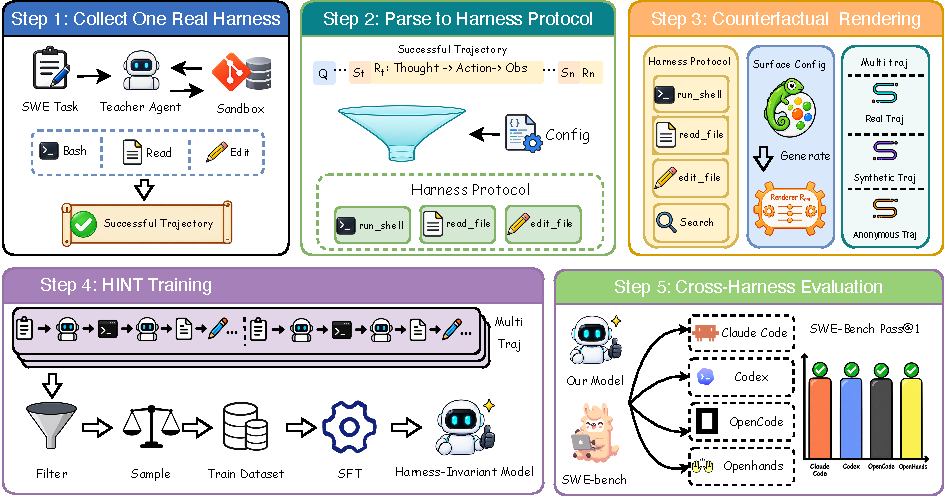
\includegraphics[width=0.85\textwidth]{pic/main_v1.pdf}
\end{center}
\caption{The \method{} pipeline: trajectories collected with a teacher agent
in one real harness are parsed down to the \HP{}, re-rendered under freshly
sampled surface configurations with real, synthetic or anonymized tool
vocabularies, filtered and sampled to a token budget, and used for
fine-tuning; the model is then evaluated under real harnesses never seen in
training.}
\label{fig:pipeline}
\end{figure}

A policy $\pi$ is \emph{interface-invariant} if its induced semantic behaviour
is unchanged by surface transport: for all $h, h'$ and all protocol states $x$,
$\tilde{\pi}\!\left(R_{h'}(x)\right) = \tilde{\pi}\!\left(R_{h}(x)\right)$, where
$\tilde\pi$ denotes the policy's output pushed back to protocol level.
Deviation from this equality is what Section~\ref{sec:exp} measures, and
\method{} is a training method that pursues it, whence its name. \method{} has
two components, counterfactual harness rendering and interface anonymization,
the second implemented as one tier of the first's name sampler; both touch
only the data, and nothing about the model architecture or the training
objective changes. Figure~\ref{fig:pipeline} traces the pipeline end to end.
\cham{}, the configurable harness we use to evaluate under synthetic surfaces,
is described with the experimental setup (Section~\ref{sec:setup}).

\subsection{Counterfactual harness rendering}
\label{sec:chr}

Given a corpus of real trajectories collected in a single harness $h_0$, we
parse each into protocol form and re-render it under $M$ configurations sampled
independently from $\mathcal{H}$:
\begin{equation}
\mathcal{D}_{\chr{}} \;=\;
\Big\{\, R_{h}\!\left(P_{h_0}(\tau)\right) \;:\;
\tau \in \mathcal{D}_{\text{real}},\;
h \sim \mathrm{Unif}(\mathcal{H}_{\mathrm{train}})^{M} \,\Big\},
\end{equation}
where $\mathcal{H}_{\mathrm{train}} \subset \mathcal{H}$ samples four axes and
fixes the call syntax $A_2$ to native function calling, so that every rendered
sample carries the \texttt{tools} schema and structured \texttt{tool\_calls}
production harnesses deploy and merges directly with ordinary agent SFT data.
The semantic content of every sample is identical to a real, verified episode;
only the surface is synthetic. This is domain randomization
\citep{tobin2017domain} applied to the agent interface rather than to visual
appearance, and two results motivate it. The domain-generalization bound of
\citet{benda2010theory} charges the divergence between training and deployment
domains, which training over a distribution of surfaces is meant to reduce.
And the identifiability assumption behind augmentation-based representation
learning, that the augmentation leaves \emph{content} untouched and perturbs
only \emph{style} \citep{kugelgen2021self}, holds here by construction and by
measurement (Proposition~\ref{prop:roundtrip}) rather than approximately as it
does for image augmentation.

\subsection{Interface anonymization}

Sampling from real vocabularies alone leaves a shortcut intact: each semantic
function has only a handful of attested names, so a model can still map
\texttt{Bash}, \texttt{bash} and \texttt{exec\_command} onto ``the shell tool''
by memorization. We therefore
draw tool names from three tiers: names harvested verbatim from real harnesses
but \emph{recombined across} them ($\approx43\%$ of samples), plausible names
that no parsed harness uses ($\approx27\%$), and meaningless pronounceable identifiers ($30\%$). The third tier is the
anonymization component: a sample drawn into it has every tool name replaced.
Canonical semantics are never anonymized: they remain in the tool
documentation, so under the third tier the documentation is the only channel
carrying the information needed to act.

\section{Experiments}
\label{sec:exp}

\subsection{Setup}
\label{sec:setup}
\paragraph{Model and data.} We fine-tune \basemodel{} \citep{qwen36card} on
$9{,}366$ \claudecode{} trajectories collected with GLM-5.3 \citep{glm53card}
as the teacher on SWE-rebench-V2 instances \citep{badertdinov2026swerebenchv2},
one per task instance; the instances are deduplicated against both evaluation
benchmarks, so no training task appears in \swev{} or \swem{}. Normalization moves every call out of the text channels, and we
check that no call text remains in the reasoning or observations of any kept
trajectory. After dropping trajectories containing unmapped tools or fewer than
three semantic actions, $8{,}677$ remain; \chr{} renders each into $M=3$
counterfactual surfaces, yielding $\numsurfaces{}$ samples, each under its own
surface configuration, with $21{,}476$ distinct tool names; $30\%$ of samples
are anonymized. The samples vary $A_1$, $A_3$, $A_4$ and $A_5$ ($10{,}335$
split, $10{,}511$ unified-editor and $5{,}185$ monolithic surfaces) and all use
native function calling. \method{} trains on these rendered samples alone. Both runs are
full-parameter fine-tuning with a global batch of $128$ packed sequences of up
to $256$K tokens and learning rate $5\times10^{-5}$ with cosine decay.

\paragraph{Step-matched control.} Rendering multiplies the data: the
rendered set holds about $1.7\times$ the tokens of the original trajectories,
so a gain could come from extra optimization rather than from surface
diversity. We therefore match optimizer steps. The \control{} trains on the
original \claudecode{} trajectories for three epochs, which is $67$ steps;
\method{} trains for the same $67$ steps, about $1.8$ passes over its rendered
set. With sequence packing, equal steps at an equal batch size are also
approximately equal training tokens. The two runs differ only in their data:
the control sees each trajectory three times in its original surface, and
\method{} sees it in three different surfaces, none of which is
\claudecode{}'s own.

\paragraph{\cham{}.} Real harnesses cannot be perturbed one axis at a time:
there is no way to give \claudecode{} \openhands{}'s observation format while
holding everything else fixed. We therefore implement \cham{}, an executable
agent harness in which every surface property is a configuration parameter
drawn from the five axes of Eq.~(\ref{eq:axes}). It parses calls, executes
them against a real workspace, and formats observations according to its
configuration, which makes it both the instrument for single-axis controlled
experiments (Section~\ref{sec:axes}) and an environment for evaluation under
arbitrary synthetic harnesses.

\paragraph{Evaluation.} We evaluate on two benchmarks and report pass@1.
\swev{} is a human-validated subset of SWE-bench \citep{jimenez2024swebench}:
$500$ tasks from $12$ Python repositories. \swem{} \citep{yang2025swesmith}
has $300$ tasks in nine other programming languages (C, C++, Go, Java,
JavaScript, TypeScript, PHP, Ruby and Rust); we refer to the two as Verified
and Multilingual. In
Sections~\ref{sec:harness-choice} and~\ref{sec:step-matched}, every model
runs under the four production harnesses of Table~\ref{tab:harnesses} and
under \cham{} with one fixed configuration, and all models are served with
vLLM \citep{kwon2023vllm} on the same serving stack;
Section~\ref{sec:harness-choice} evaluates three open-weight models,
Qwen3.5-35B-A3B \citep{qwen35card}, \basemodel{} and KAT-Coder-V2.5-Dev
\citep{huang2026katcoder}, once per cell, and Section~\ref{sec:step-matched}
evaluates the two fine-tuned models and averages three evaluations per cell.
The later experiments state their own conditions. We call \opencode{},
\openhands{} and \codexcli{} unseen because training never presented any of
them as a coherent harness; Section~\ref{sec:limits} counts the rendered
samples that carry one of their tool names. Appendix~\ref{app:eval} gives the run-to-run noise floor and summarizes the
settings of every experiment in Table~\ref{tab:settings}.

\subsection{Harness choice alone}
\label{sec:harness-choice}

\begin{table}[t]
\caption{Harness choice alone moves accuracy. Pass@1 (\%) of three open-weight
models on \swev{} (V, $500$ tasks) and \swem{} (M, $300$ tasks) under the four
production harnesses and \cham{} (one fixed configuration), one evaluation per
cell. Spread is max minus min over the five harnesses.}
\label{tab:e0}
\begin{center}
\begin{small}
\setlength{\tabcolsep}{4pt}
\begin{tabular}{@{}l S[table-format=2.1, table-fixed-width=true, table-column-width=38pt] S[table-format=2.1, table-fixed-width=true, table-column-width=38pt] @{\hspace{12pt}} S[table-format=2.1, table-fixed-width=true, table-column-width=38pt] S[table-format=2.1, table-fixed-width=true, table-column-width=38pt] @{\hspace{12pt}} S[table-format=2.1, table-fixed-width=true, table-column-width=38pt] S[table-format=2.1, table-fixed-width=true, table-column-width=38pt]@{}}
\toprule
 & \multicolumn{2}{c}{Qwen3.5-35B-A3B} & \multicolumn{2}{c}{\basemodel{}} & \multicolumn{2}{c}{KAT-Coder-V2.5-Dev} \\
\cmidrule(r){2-3}\cmidrule(lr){4-5}\cmidrule(l){6-7}
Harness & {V} & {M} & {V} & {M} & {V} & {M} \\
\midrule
\claudecode{} & 64.2 & 54.7 & 69.0 & 62.3 & 69.4 & 57.3 \\
\opencode{}   & 66.4 & 54.3 & 71.4 & 68.3 & 69.8 & 58.7 \\
\openhands{}  & 67.6 & 58.3 & 71.0 & 64.3 & 68.8 & 60.3 \\
\codexcli{}   & 58.6 & 49.7 & 68.0 & 61.3 & 68.6 & 59.3 \\
\cham{}       & 67.2 & 55.0 & 70.8 & 62.3 & 67.2 & 60.0 \\
\midrule
Spread        & 9.0  & 8.7  & 3.4  & 7.0  & 2.6  & 3.0  \\
\bottomrule
\end{tabular}
\end{small}
\end{center}
\end{table}

Table~\ref{tab:e0} establishes the phenomenon the method addresses. The ordering
is not explained by tool count or interface simplicity: \codexcli{}, which
declares $13$ tools but routes file operations through a shell, is the lowest
of the four production harnesses on Verified for all three open-weight models,
while \openhands{}, with $4$ tools, is the best or second best harness for the
two Qwen models. The size of the spread is a property of the model: $9.0$
points for Qwen3.5-35B-A3B, $3.4$ for \basemodel{} and $2.6$ for
KAT-Coder-V2.5-Dev on Verified, in the same order on Multilingual ($8.7$,
$7.0$, $3.0$). KAT-Coder-V2.5-Dev, which was post-trained with harness randomization
\citep{huang2026katcoder}, shows the smallest spread of the three; \method{}
aims to obtain the same property from the training data alone.

\subsection{\method{} versus a step-matched control}
\label{sec:step-matched}

\begin{table}[t]
\caption{\method{} versus the \control{}, both fine-tuned from \basemodel{}:
pass@1 (\%) on \swev{} and \swem{}. Fine-tuned cells are means of three
evaluations; Base is the model before fine-tuning (Table~\ref{tab:e0}).
$\Delta$ is \method{} minus control, and bold marks the better of the two (the
lower, for spread). Mean, worst and spread are taken over the five harnesses;
the noise floor of a single evaluation is $\pm2.0$ on Verified and $\pm1.0$ on
Multilingual.}
\label{tab:e1}
\begin{center}
\begin{small}
\setlength{\tabcolsep}{4.5pt}
\begin{tabular}{@{}l S[table-format=2.1] S[table-format=2.1] S[table-format=2.1] S[table-format=+1.1] @{\hspace{16pt}} S[table-format=2.1] S[table-format=2.1] S[table-format=2.1] S[table-format=+1.1]@{}}
\toprule
 & \multicolumn{4}{c}{\swev{}} & \multicolumn{4}{c}{\swem{}} \\
\cmidrule(r){2-5}\cmidrule(l){6-9}
Harness & {Base} & {Control} & {\method{}} & {$\Delta$} & {Base} & {Control} & {\method{}} & {$\Delta$} \\
\midrule
\claudecode{} (source) & 69.0 & 78.4 & \bfseries 78.6 & +0.2 & 62.3 & 68.7 & \bfseries 75.0 & +6.3 \\
\opencode{}            & 71.4 & 74.3 & \bfseries 77.1 & +2.8 & 68.3 & 71.9 & \bfseries 73.4 & +1.5 \\
\openhands{}           & 71.0 & 77.2 & \bfseries 81.7 & +4.5 & 64.3 & 71.7 & \bfseries 74.0 & +2.3 \\
\codexcli{}            & 68.0 & 66.7 & \bfseries 75.4 & +8.7 & 61.3 & 66.0 & \bfseries 73.4 & +7.4 \\
\cham{}                & 70.8 & \bfseries 78.4 & 75.6 & -2.8 & 62.3 & 73.4 & \bfseries 74.4 & +1.0 \\
\midrule
Mean                   & 70.0 & 75.0 & \bfseries 77.7 & +2.7 & 63.7 & 70.3 & \bfseries 74.0 & +3.7 \\
Worst                  & 68.0 & 66.7 & \bfseries 75.4 & +8.7 & 61.3 & 66.0 & \bfseries 73.4 & +7.4 \\
Spread                 & 3.4  & 11.7 & \bfseries 6.3  & -5.4 & 7.0  & 7.4  & \bfseries 1.6  & -5.8 \\
\bottomrule
\end{tabular}
\end{small}
\end{center}
\end{table}

\begin{figure}[t]
\begin{center}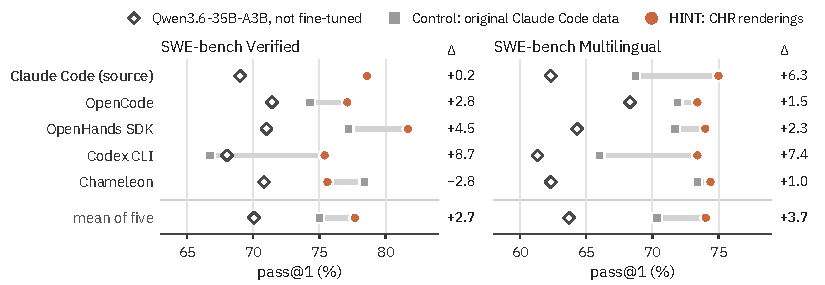
\includegraphics[width=\textwidth]{pic/e1_step_matched.pdf}
\end{center}
\caption{Table~\ref{tab:e1} by harness. Each row places the base model (open
diamond), the control (grey square) and \method{} (orange circle); the bar
joins the two fine-tuned models, and the number to its right is \method{} minus
control, grey when within the single-evaluation noise floor. On Verified the
control's gain over the base model is largest on its source harness and
vanishes on \codexcli{}; \method{}'s gain is spread across harnesses, and on
Multilingual its five accuracies lie within $1.6$ points.}
\label{fig:e1}
\end{figure}

Table~\ref{tab:e1} and Figure~\ref{fig:e1} give the result. Both fine-tuned
models improve on the base model on average, the control by $5.0$ points on
Verified and $6.6$ on Multilingual, \method{} by $7.6$ and $10.3$. Where the control's gain lands illustrates the problem of
Section~\ref{sec:intro}.
On Verified it gains $9.4$ points under \claudecode{}, the harness its data came
from, $2.9$ under \opencode{}, and less than the noise floor under \codexcli{}
($68.0\%$ before fine-tuning, $66.7\%$ after), so its spread across harnesses grows from $3.4$
to $11.7$ points. Fine-tuning on one harness raised accuracy on that harness and made the model
more dependent on it.

On the source harness \method{} is level with the control on Verified
($78.6\%$ against $78.4\%$, within the noise floor) and ahead on Multilingual
($75.0\%$ against $68.7\%$), although it never trained on \claudecode{}'s own
surface. Under the three unseen production
harnesses it is ahead on both benchmarks, by $2.8$, $4.5$ and $8.7$ points on
Verified and by $1.5$, $2.3$ and $7.4$ on Multilingual. The largest gap is under
\codexcli{}, whose shell-only surface lies outside the surfaces \chr{} renders
for training (Section~\ref{sec:limits}). The advantage is therefore largest where the control is weakest:
\method{}'s worst harness is $8.7$ points (Verified) and $7.4$ points
(Multilingual) above the control's, and on Multilingual its five accuracies lie
within $1.6$ points ($73.4$--$75.0\%$), a tighter range than the base model's
own $7.0$. Against the single-evaluation noise floor (Appendix~\ref{app:eval}), \method{} is ahead in
seven of the ten cells, level in two (\claudecode{} on Verified, \cham{} on
Multilingual), and behind in one.

That one cell is \cham{} on Verified, where the control leads by $2.8$ points
($78.4\%$ against $75.6\%$). \cham{}'s configuration comes from the space
\method{}'s training surfaces were sampled from, so this is not a failure to
reach an unseen surface of the kind the other production-harness rows measure, and we do not
have an explanation for it. An earlier run of the same comparison on a weaker
base model with a different recipe is reported in Appendix~\ref{app:e1-30b};
there \method{}'s advantage appeared on Multilingual only.

\subsection{Real trajectories from more harnesses}
\label{sec:real}

\begin{figure}[t]
\begin{center}
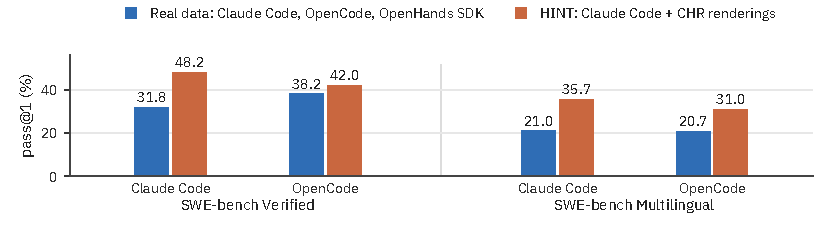
\includegraphics[width=\textwidth]{pic/real_harness_data.pdf}
\end{center}
\caption{\method{} versus a model trained on real trajectories from four harnesses, both fine-tuned from \oldmodel{} for the same
number of steps, under the four production harnesses and \cham{} (pass@1, one
evaluation per cell). \textbf{(a)}~\swev{}. \textbf{(b)}~\swem{}.}
\label{fig:real}
\end{figure}

A direct alternative to rendering counterfactual surfaces is to collect real
trajectories in several harnesses, and we compare the two on
\oldmodel{}, the base model of Appendix~\ref{app:e1-30b}. The \method{} model of that appendix trains on \claudecode{} trajectories
mixed with their \chr{} renderings. The alternative trains on real
trajectories collected in four harnesses, \claudecode{}, \opencode{},
\openhands{} and \codexcli{}, with the same schedule and the same number of
optimizer steps. Both models are evaluated under the four production harnesses
and \cham{}, once per cell. Four of the five surfaces occur in the training
data of the model trained on real trajectories, and only \cham{} is unseen for
it, whereas for \method{} every surface but \claudecode{} is unseen.
As Figure~\ref{fig:real} shows, \method{} is ahead under \claudecode{},
$48.2\%$ against $31.8\%$ on Verified and $35.7\%$ against $21.0\%$ on
Multilingual, and under \opencode{}, by $3.8$ points on Verified ($42.0\%$
against $38.2\%$) and $10.3$ on Multilingual ($31.0\%$ against $20.7\%$),
although the other model trained on \opencode{} trajectories. Under
\openhands{} and \codexcli{}, both in that model's training data, and under
\cham{}, the two are within a few points of each other: $58.4\%$ against
$54.0\%$ and $44.7\%$ against $43.3\%$ under \openhands{}, $40.2\%$ against
$37.1\%$ and $22.6\%$ against $24.4\%$ under \codexcli{}, and $42.4\%$
against $40.2\%$ and $26.0\%$ against $24.0\%$ under \cham{}. Averaged over
the five harnesses \method{} is $2.1$ points higher on Verified and $4.7$ on
Multilingual, and its accuracy varies across harnesses by $16.9$ and $19.3$
points against the other model's $26.6$ and $24.0$. At an equal step budget,
then, training data whose surfaces are synthetic performs on a par with real
trajectories distilled in the target harnesses themselves: \method{} is ahead
under two of the four harnesses the other model trained in, within a few
points under the other two and under \cham{}, and higher on average. The two
training sets also differ in their tasks, so the comparison is between two
data pipelines rather than between surfaces alone.

\subsection{Test-time anonymization of the interface}
\label{sec:anon}

\begin{figure}[t]
\begin{center}
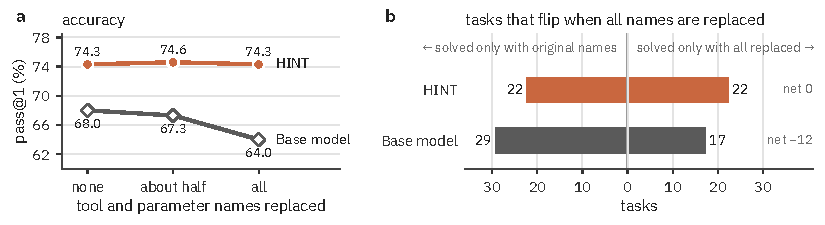
\includegraphics[width=\textwidth]{pic/anon_names.pdf}
\end{center}
\caption{Anonymizing tool and parameter names under \cham{} on \swem{}, for
\basemodel{} before fine-tuning and the \method{} model of Table~\ref{tab:e1},
one evaluation per setting. \textbf{(a)}~Pass@1 as more names are replaced.
\textbf{(b)}~Tasks whose outcome flips when all names are replaced.}
\label{fig:anon}
\end{figure}

Whole harnesses differ from the training surfaces in many respects at once, so
they cannot show which cue a model relies on. We isolate the cheapest cue, the identifiers of tools and their parameters,
which let a model that recognizes \texttt{Bash} act without reading its
description and which \chr{}'s anonymized tier is meant to make
unnecessary. Holding the
\cham{} configuration of Table~\ref{tab:e0} fixed ($9$ tools with $17$
parameters), we replace about half of the tool and parameter names ($4$ and
$8$, respectively), and then all of them, with meaningless identifiers, so
that, for example, \texttt{run\_command} becomes \texttt{zete}. The tool
descriptions are identical across settings and the system prompt names no
tool, so what each tool does remains readable throughout. \basemodel{} before
fine-tuning and the \method{} model of Table~\ref{tab:e1} are each evaluated
once per setting on \swem{} and compared only with their own run under the
original names; because these runs are separate from those of
Tables~\ref{tab:e0} and~\ref{tab:e1}, only differences
between settings are interpreted. As Figure~\ref{fig:anon} shows, \method{}'s
accuracy is unchanged ($74.3\%$, $74.6\%$ and $74.3\%$), and with all names
replaced it newly fails exactly as many tasks as it newly solves ($22$ each).
The base model falls from $68.0\%$ to $67.3\%$ and $64.0\%$, losing $29$ tasks
and gaining $17$, and its additional failures coincide with the new identifiers: calls to tools
that do not exist rise from $5$ to $27$ of the $300$ tasks, and the calls
misspell the new identifiers (\texttt{kazu\_op} for
\texttt{kozu\_op}) rather than revert to the original ones. On this interface, then, \method{}'s accuracy does not depend on recognizable
identifiers, which is the behaviour the anonymized tier is meant to teach; the
$22$ tasks that flip in each direction show that individual episodes still
change. The test
is nonetheless in distribution: \method{}'s training data was anonymized with
the same identifier generator, so the result shows that this behaviour was
acquired, not that it extends to naming schemes unseen in training.

\subsection{One surface axis at a time}
\label{sec:axes}

\begin{figure}[t]
\begin{center}
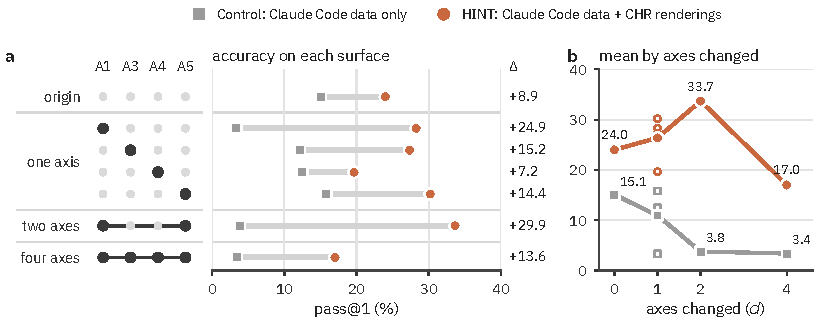
\includegraphics[width=\textwidth]{pic/chameleon_axes.pdf}
\end{center}
\caption{\cham{} surfaces that move surface axes, one or several at a time,
away from a \claudecode{}-like origin (\swem{}, one evaluation per surface).
\textbf{(a)}~The axes each surface changes (A1 naming and granularity, A3 prompt
and documentation, A4 observation format, A5 turn conventions) and the accuracy
of \method{} and of the control; $\Delta$ is \method{} minus control.
\textbf{(b)}~Mean accuracy over the surfaces that change $d$ axes (one surface
each at $d=0$, $2$ and $4$); open markers are the four single-axis surfaces.}
\label{fig:axes}
\end{figure}

Production harnesses differ on several surface axes at once, so
Section~\ref{sec:step-matched} cannot say which axis a model is bound to, and
Section~\ref{sec:anon} isolates only one cue; \cham{} can move the axes one at
a time. We start from an origin
configuration that mimics \claudecode{}, with its split tools and their names
and parameters, an engineering system prompt with formal tool documentation,
numbered file views and \claudecode{}'s turn conventions, and move each axis in turn to a pre-selected far setting. A1 merges the tools into a single monolithic tool
with anonymized tool and parameter names; A3 changes the persona of the system
prompt and renders the tool documentation as tables; A4 drops line numbers,
wraps observations in a fence, truncates them at $2{,}000$ characters and
changes the markers for empty and failed output; A5 removes the runtime
reminder, adds a turn header, returns observations as user turns and ends an
episode with a finish call. Two further surfaces change A1 and A5 together and
all four axes. The call syntax (A2) is fixed by native function calling, and
every surface exposes the same actions. We evaluate the \method{} model of
Appendix~\ref{app:e1-30b} and a control fine-tuned from the same base model,
\oldmodel{}, on the same \claudecode{} trajectories alone, once
per surface on \swem{}. These runs use a different evaluation environment from
Appendix~\ref{app:e1-30b} and exclude the few episodes
still running when a cell was closed (at most $15$ of $300$), so their absolute
accuracies are not comparable with Table~\ref{tab:e1-30b} and only differences
between surfaces are interpreted. The control is bound to A1 (Figure~\ref{fig:axes}a): changing
naming and granularity alone takes it from $15.1\%$ on the origin to $3.3\%$,
and it stays at that level whenever A1 is changed ($3.8\%$ with A1 and A5,
$3.4\%$ with all four axes), whereas changing A3, A4 or A5 alone leaves it
between $12.2\%$ and $15.8\%$. \method{} is not: with A1 changed alone it scores
$28.3\%$ against $24.0\%$ on the origin, and with A1 and A5 changed together
$33.7\%$; only the surface that changes all four axes brings it down, to
$17.0\%$. \method{} is ahead of the control on every surface, by $8.9$ points on
the origin and by $29.9$ points when A1 and A5 are changed together, and
averaged over the surfaces at each distance from the origin (one surface each
at $d=0$, $2$ and $4$, four at $d=1$) its accuracy is $24.0\%$, $26.4\%$,
$33.7\%$ and $17.0\%$ for $d=0$, $1$, $2$ and $4$, against
$15.1\%$, $11.0\%$, $3.8\%$ and $3.4\%$ for the control
(Figure~\ref{fig:axes}b). A model trained on one harness has thus absorbed that
harness's tool vocabulary and granularity as part of the task, which \method{}
has not; what remains for \method{} is a loss when every axis changes at once.

\section{Limitations}
\label{sec:limits}

Each experiment uses one base model and one source harness, and each
fine-tuned model is a single training run compared against a noise floor
rather than across repeated training. Because \chr{}'s first naming tier
recombines real tool names, $33\%$ of the rendered samples carry a
\claudecode{} name, $33\%$ an \opencode{} name and $21\%$ a \codexcli{} name,
while none carries an \openhands{} name or presents any held-out harness as a
coherent whole; the held-out harnesses are therefore unseen as interfaces, not
as vocabularies. Training surfaces keep first-class file tools, so a shell-only
surface such as \codexcli{}'s is never rendered into training data. Whether the
effect scales with model size, holds for a shell-only source harness, or
separates into the contributions of surface diversity and anonymization
remains open.

\section{Related work}
\label{sec:related}

\paragraph{SWE agents, scaffolds and their training data.}
\citet{jimenez2024swebench} established the benchmark, and
\citet{yang2024sweagent} showed that the agent--computer interface itself
materially determines performance. Scaffolds since then range from a pipeline
or a bare shell \citep{xia2024agentless,minisweagent2025} to the rich tool sets
of OpenHands \citep{wang2025openhands,wang2025openhandssdk} and of the
production harnesses we study \citep{anthropic2025claudecode,openai2025codex,
opencode2025}, and recent measurements confirm that the choice among them is a
first-order factor: it moves scores by as much as the choice of model
\citep{zhang2026stopcomparing,yao2026harnessbench,zheng2026clawswebench}, the
two shares vary across benchmarks \citep{merrill2026terminalbench}, and
single-run differences of a few points lie within evaluation noise
\citep{bjarnason2026randomness}. On the training side, SWE-Gym
\citep{pan2024swegym}, SWE-smith \citep{yang2025swesmith}, R2E-Gym
\citep{jain2025r2egym}, SWE-rebench
\citep{badertdinov2025swerebench,badertdinov2026swerebenchv2}, Skywork-SWE
\citep{zeng2025skyworkswe} and Devstral \citep{rastogi2025devstral} scale tasks
and trajectories within one scaffold, while a growing line of work trains
across many: mixing real trajectories from several scaffolds
\citep{abadji2026laguna}, randomizing synthetic tool sets or environments
\citep{kimiteam2025k2,chen2026minimaxm2,cao2026qwen3codernext}, or randomizing
the harness during reinforcement learning
\citep{huang2026katcoder,xu2026polar,yu2026openforgerl}. Those works vary the
scaffold at evaluation time or collect trajectories in every harness; we treat
the scaffold as a nuisance variable at training time and are, to our
knowledge, the first to synthesize its surfaces by re-rendering one harness's
real trajectories, and Section~\ref{sec:real} compares the two directly.

\paragraph{Interface reliance, invariance and protocol representations.}
\citet{gu2026interfaces} show with semantics-preserving renaming that
trajectory SFT amplifies interface memorization over semantic understanding,
\citet{may2026runtime} that agents internalize runtime conventions, and
prompt-format sensitivity \citep{sclar2023sensitivity} and the loss of
generalization under a frozen prompt template \citep{lin2025debunk} are the
same phenomenon at the prompt level; diversity of tool settings
\citep{he2025gentool} and function masking against name memorization
\citep{lin2024hammer} are precursors of \chr{}'s naming tiers and
anonymization. The remedy we adopt is domain randomization
\citep{tobin2017domain} rather than a penalty as in invariant risk
minimization \citep{arjovsky2019irm}, and the bound of \citet{benda2010theory}
formalizes why exposure to a distribution of domains helps; our setting is
unusually favourable to this family of methods, because the content-preserving
property that \citet{kugelgen2021self} must assume of an augmentation is here
measured at \rtacc{}, and the transformations between surfaces are explicit
and composable rather than latent \citep{higgins2018symmetry}. The Agent Data
Protocol \citep{song2025adp} also defines a scaffold-independent trajectory
representation and compiles it into several scaffolds' SFT formats; our
protocol differs in being recovered from production harnesses by
normalization, in factoring the surface into axes that are sampled rather than
compiled to fixed targets, and in an invertibility that is proved and
measured, with the algebraic reading of the protocol as a normal form
following \citet{allen2019analogies}.

\section{Conclusion}

Agent harnesses differ far more on the surface than in substance: four
production harnesses, ranging from $4$ tools to $21$ and from
first-class file editors to file access through a shell alone, reduce to $12$ semantic
actions covering $99.96\%$ of $\numactions{}$ real calls. Making that core explicit
as the \HP{}, and verifying that the surface map is invertible on those calls,
exactly in $95.2\%$ of \numroundtrip{} render--parse checks and up to an
operational equivalence in the rest, turns interface variation into something a
training pipeline can marginalize over. \method{} does so with no new task data and no
architectural change: at an equal number of training steps it matches a single-harness control on
that control's harness, and is ahead of it under every
unseen production harness, by up to $8.7$ points. Aligning hidden
representations across renderings of the same decision point, which
Proposition~1 makes well posed, is the natural next step.

\subsection*{AI use statement}

In this work, we used generative AI tools for editing and polishing the text
of the manuscript, that is, for improving grammar, wording and readability of
sentences that we wrote. We have not used generative AI tools for research
ideation, for the design of the method or of the experiments, for writing the
code of the renderer, the harness or the evaluation pipeline, or for producing
or analysing the data and results reported here, and the remaining tasks with
required disclosure are not applicable to this work. We have reviewed all
AI-assisted text. We take responsibility for the final content of this work,
including any text produced with the aid of generative AI.

\subsection*{Ethics statement}

This work trains and evaluates software-engineering agents on public GitHub
repositories: the training tasks are SWE-rebench-V2 instances and the
evaluation tasks are the public \swev{} and \swem{} sets. No human subjects,
personal data or code beyond these public repositories are involved, and
repository content is used under its own licenses. Trajectories are collected
and evaluated in isolated sandboxes that cannot affect systems outside the task
container. The method aims to make agents less sensitive to their interface, and
we foresee no harm specific to it beyond those of coding agents in general.

\subsection*{Reproducibility statement}

Section~\ref{sec:protocol} and Appendix~\ref{app:proof} define the protocol,
the renderer and the parser, state the premises (P1)--(P4) and prove
Proposition~1; the round-trip check that verifies the implementation is
described in Section~\ref{sec:protocol} and Table~\ref{tab:roundtrip}, with
the $\simeq$ cases enumerated in Appendix~\ref{app:premises}.
Section~\ref{sec:method} specifies the training-surface space
$\mathcal{H}_{\mathrm{train}}$ and the three naming tiers, and
Section~\ref{sec:setup} gives the task source, teacher, filters, sample
counts, per-axis composition and training hyperparameters of both fine-tuning
runs. Appendix~\ref{app:eval} lists every experiment's models, harnesses,
evaluation counts and conditions (Table~\ref{tab:settings}), the rounding
rule, the noise floor and the harness releases evaluated. We plan to release the parsers, the renderer, the \cham{} harness,
the surface sampler and the evaluation configurations, together with the
rendered training samples, as supplementary material.

\bibliography{hint}
\bibliographystyle{iclr2027_conference}

\appendix
\section{Proof of Proposition 1}
\label{app:proof}

Proposition~1 states that the surface map of every harness our renderer
realizes is exactly invertible on the action channel. The proof is by
construction: the renderer is a composition of two stages, and each stage is
shown to have a left inverse. Section~\ref{app:setting} fixes notation,
Sections~\ref{app:naming}--\ref{app:shell} prove one lemma per stage,
Section~\ref{app:theorem} assembles them, Section~\ref{app:premises}
lists the premises and states precisely what the measurement of
Table~\ref{tab:roundtrip} adds to the proof, and Section~\ref{app:orbit}
illustrates the construction on one trajectory.

\subsection{Setting}
\label{app:setting}

\paragraph{Actions.} An action is a pair $a=(v,r)$ of a \emph{verb}
$v\in\mathcal{V}$ and a \emph{record} $r$. The verb set $\mathcal{V}$ has the
twelve elements of Table~\ref{tab:vocab} (the four \texttt{edit\_file}
sub-actions count as distinct verbs). Every verb has a finite set of parameter
keys $K_v$, each with a declared type (string, integer, boolean, or JSON
value); a record is a partial map $r:K_v\rightharpoonup \mathbb{V}$ from keys to
values of the declared type. Unset keys are simply absent; two records are
equal when they are equal as partial maps. $\mathcal{A}$ is the set of all such
pairs.

\paragraph{Configurations.} Of the five axes of Eq.~(\ref{eq:axes}), only
$A_1$ and $A_2$ touch the text of a call. A configuration $h$ contributes
\begin{itemize}
\item a granularity $g\in\{\textsc{split},\textsc{unified},\textsc{mono}\}$,
      which fixes the set $T_g$ of surface tools: twelve tools, one per verb;
      eight tools, one \emph{editor} tool shared by the five file verbs; or a
      single tool;
\item a tool-name map $N:T_g\to\Sigma^{*}$ and a parameter-name map
      $\Pi:K\to\Sigma^{*}$, where $K$ is the union of all $K_v$ together with
      the \emph{selector} keys of the editor and the single tool;
\item a syntax family $s\in\{\textsc{json},\textsc{xml},\textsc{yaml},
      \textsc{shell}\}$.
\end{itemize}
The remaining components (prompt template, documentation style, observation
decoration, turn conventions) are constant with respect to the action text and
play no role below.

\paragraph{Factorization.} On one action the renderer is
$R_h = E_s\circ N_h$, where the naming stage $N_h$ maps an action to a
\emph{named record} $(n,\rho)$ (a surface tool name and a record over surface
parameter names) and the syntax stage $E_s$ serializes the named record to
text. The parser is $P_h = N_h^{-1}\circ D_s$ with $D_s$ the block decoder of
the family. The shell family has no named tools and defines $E_{\textsc{shell}}$
directly on actions (Section~\ref{app:shell}). All four families share an
\emph{escape encoding} $E_{\mathrm{esc}}(a)$: a fenced block tagged
\texttt{call} whose single line is the JSON serialization of
$\{\texttt{action}:v,\ \texttt{args}:r\}$ with the canonical verb and keys.
Since JSON escapes newlines, the payload occupies one line and the closing
fence is unambiguous, so $E_{\mathrm{esc}}$ is decoded exactly by reading the
fence and applying the JSON parser. Every use of $E_{\mathrm{esc}}$ below is
therefore exact and bypasses the naming stage.

\paragraph{Premises.} The lemmas use four premises, each discharged in
Section~\ref{app:premises}:
\begin{itemize}
\item[(P1)] $N$ is injective on $T_g$;
\item[(P2)] $\Pi$ is injective on the key set of each surface tool;
\item[(P3)] (\textsc{json} only) no argument value contains a well-formed call of
      the same configuration;
\item[(P4)] values carry their declared types, and a string-valued JSON
      parameter is not itself a JSON document.
\end{itemize}

\subsection{Lemma 1: the naming stage is an injective table lookup}
\label{app:naming}

\begin{lemma}\label{lem:naming}
Under (P1), (P2) and (P4), $N_h$ is injective and the
inverse tables of the parser recover $(v,r)$ from $(n,\rho)$.
\end{lemma}
\begin{proof}
Let $\tau:\mathcal{V}\to T_g$ assign each verb its surface tool.
Under \textsc{split}, $\tau$ is a bijection and $N_h(v,r)=(N(\tau(v)),\
r\circ\Pi^{-1})$. Under \textsc{unified}, the five file verbs share the editor
tool, and $N_h$ adds to the renamed record one selector entry
$\Pi(\mathrm{sel})\mapsto\ell(v)$ with $\ell$ an injection of the five verbs
into the literals $\{\texttt{view},\texttt{str\_replace},\texttt{insert},
\texttt{create},\texttt{undo\_edit}\}$; all other verbs are treated as under
\textsc{split}. Under \textsc{mono}, every verb uses the single tool and the
selector carries one of twelve distinct literals. In each case the decoder
proceeds in three steps. (i) From $n$ it recovers the surface tool, because $N$
is injective (P1). (ii) If the tool is the editor or the single tool, it reads
the selector entry, which is present because the encoder always writes it and
unambiguous because the selector key is distinct from every data key of that
tool (P2); the literal determines $v$ because $\ell$ is injective. Otherwise
the tool determines $v$ because $\tau$ is a bijection on the remaining verbs.
(iii) It renames the data keys back through $\Pi^{-1}$, which is well defined
on the tool's key set by (P2), and re-types the values by the declared type
of each key, which returns the original values by (P4). Hence the decoder is a
left inverse of $N_h$ and $N_h$ is injective.
\end{proof}

\subsection{Lemma 2: the named-tool syntax families are decodable encodings}
\label{app:named}

\begin{lemma}\label{lem:named}
For $s\in\{\textup{\textsc{json}},\textup{\textsc{xml}},\textup{\textsc{yaml}}\}$
and every named record $(n,\rho)$, $D_s(E_s(n,\rho))=(n,\rho)$; for
\textup{\textsc{json}} this uses (P3).
\end{lemma}
\begin{proof}
Write $J$ for JSON serialization. $J$ is injective on finite
records with distinct string keys and values of the types above (every string
becomes a quoted string in which quotes, backslashes and control characters
are escaped), and $J^{-1}\circ J$ is the identity on them.

\textsc{json}: $E(n,\rho)$ is $J(\{\texttt{name}:n,\texttt{arguments}:\rho\})$
between an opening and a closing tag. $D$ scans for the opening tag, takes the
first brace after it and the shortest prefix that is a balanced object under a
string-aware bracket count, and applies $J^{-1}$. The output of $J$ is itself
such a balanced object, and braces inside its string literals are skipped by
the string-aware count, so the recovered prefix is exactly $J$'s output. A tag
occurring inside a value can only start a second candidate block; by (P3) that
block is not a well-formed call of the configuration and is rejected, so the
decoder returns the single record. In the structured tool-calling channel used
for training, the object is carried by the API rather than located by tag
scanning, and (P3) is not needed.

\textsc{xml}: if any value contains a closing marker of the family
(\texttt{</arg>}, \texttt{</invoke>}, or the opening of an invoke element),
$E$ routes the action to $E_{\mathrm{esc}}$, which is exact. Otherwise $E$
writes an invoke element carrying $n$ and, per key, an \texttt{arg} element
carrying the value: strings verbatim, other types as $J(\cdot)$. $D$ takes the
shortest span from the opening element to \texttt{</invoke>} and, inside it,
the shortest span from each \texttt{arg} opening to the next \texttt{</arg>}.
Because no value contains these markers, both spans are the intended ones;
newlines are matched, so strings come back verbatim, and non-string values are
recovered by $J^{-1}$ followed by re-typing (P4).

\textsc{yaml}: $E$ opens a fence tagged \texttt{action}, writes
\texttt{tool:} $n$, then one line per key. A value that is not a multi-line
string is written on the key's own line as $J(\cdot)$; a multi-line string is
written as a block scalar (\texttt{|-}) whose lines follow, each prefixed by
exactly four spaces, an empty line becoming four spaces. The fence closes at
column~0. No value can produce a line starting at column~0: single-line values
are on the key line with newlines escaped by $J$, and block lines are indented.
Hence the first column-0 fence after the opening is the true end of the block.
$D$ reads key lines at two spaces of indentation, collects the four-space lines
of a block scalar while stripping the prefix, and drops trailing lines that are
genuinely empty; the only such line is the one produced by the newline before
the closing fence, since empty value lines were encoded as four spaces. Scalars
on key lines are recovered by $J^{-1}$.
\end{proof}

\subsection{Lemma 3: the shell-only family is exact up to $\simeq$}
\label{app:shell}

The \textsc{shell} family has no named tools, so the naming stage is empty and
$E_{\textsc{shell}}$ is defined verb by verb. Some verbs have no surface form of
their own in this family and are \emph{lowered} to the shell command that
performs them; the decoder then returns that command. This is the one place
where the round trip is not literally the identity, and we make the slack
explicit.

\paragraph{Operational equivalence.} Write $a\simeq a'$ when the two actions
induce the same environment transition and the same observation content, with
decoration removed, from every workspace state. The relation identifies:
a file read with the shell command that performs it,
$\texttt{read\_file}(p,s,e)\simeq\texttt{run\_shell}(\texttt{sed -n
\textquotesingle s,ep\textquotesingle{} }p)$ and $\texttt{read\_file}(p)\simeq\texttt{run\_shell}(\texttt{cat
}p)$; a search with the corresponding \texttt{grep} or \texttt{find}
command; a fetch with \texttt{curl}; two shell commands that differ only in
leading or trailing newlines; a submission whose message is empty with the
documented filler message; and an action with an argument the executor
ignores (the display label of a delegation, the \texttt{view}/\texttt{plan}
selector of a task-list update) with the same action without it.

\begin{lemma}\label{lem:shell}
For every action $a$,
$P_{\textup{\textsc{shell}}}(E_{\textup{\textsc{shell}}}(a))\simeq a$. Consequently
$E_{\textup{\textsc{shell}}}(a)=E_{\textup{\textsc{shell}}}(a')$ implies $a\simeq a'$.
\end{lemma}
\begin{proof}
We list the encoding and its decoding per verb.
\texttt{run\_shell}: the command in a fenced block tagged \texttt{bash}; a
command containing a fence goes to $E_{\mathrm{esc}}$. The decoder takes the
shortest span to the closing fence and strips outer newlines ($\simeq$).
\texttt{edit\_file}: a patch envelope. The header line carries the path, so a
path that is empty, contains a newline, has outer whitespace, or contains the
envelope terminator goes to $E_{\mathrm{esc}}$; the body carries the old and
new text line by line, each line prefixed by \texttt{-} or \texttt{+}, so any
content is expressible except one containing the terminator itself, which
goes to $E_{\mathrm{esc}}$. Insertion adds \texttt{@@ after line $k$} to the
header, creation uses an \texttt{Add File} header with \texttt{+} lines,
undo a \texttt{Revert Last Edit} header, and a replace-all edit, which no patch
expresses, goes to $E_{\mathrm{esc}}$. The decoder inverts each form line by
line and is exact. \texttt{delegate}: an envelope whose header carries the
agent kind and whose body carries the prompt verbatim (the terminator inside
the prompt goes to $E_{\mathrm{esc}}$); the display label is dropped
($\simeq$). \texttt{task\_track}: a \texttt{PLAN UPDATE} block whose body,
the list serialized by $J$ when structured, runs to the next block; a body
containing a block opener goes to $E_{\mathrm{esc}}$; the selector is dropped
($\simeq$). \texttt{web\_search}, and \texttt{web\_fetch} with an extraction
prompt: $E_{\mathrm{esc}}$, exact. \texttt{read\_file}, \texttt{search} and
\texttt{web\_fetch} without a prompt: lowered to \texttt{sed}/\texttt{cat},
\texttt{grep}/\texttt{find} and \texttt{curl} commands inside a \texttt{bash}
fence, decoded as \texttt{run\_shell} ($\simeq$). \texttt{submit}: the message
as plain text; a message that is empty or whitespace becomes the filler
($\simeq$), and one containing a block opener goes to $E_{\mathrm{esc}}$. The
decoder collects fences, escape blocks, patch and delegation envelopes and the
plan block, keeps the earliest non-overlapping ones so that a fence quoted
inside a patch body is not a second call, and reads block-free text as a
submission. In every case the decoded action is the original or its
$\simeq$-image, which proves the first claim; the second follows because
$\simeq$-images are unique up to $\simeq$.
\end{proof}

\subsection{Proof of the proposition}
\label{app:theorem}

\begin{proof}[Proof of Proposition~\ref{prop:roundtrip}]
For a configuration with a named-tool family, Lemmas~1 and~2 give
$P_h\circ R_h = N_h^{-1}\circ D_s\circ E_s\circ N_h = N_h^{-1}\circ N_h =
\mathrm{id}$ on $\mathcal{A}$. For the shell family, Lemma~3 gives
$P_h\circ R_h\simeq\mathrm{id}$. A map with a left inverse is injective, so
$R_h$ is injective on actions, modulo $\simeq$ in the shell case. The
trajectory-level statement follows step by step: an assistant turn is the
reasoning text followed by the call blocks of that step, separated by blank
lines, and the decoder returns the text outside the blocks as the reasoning.
This is exact as long as the reasoning contains no block opener of the family,
which the normalization of Section~\ref{sec:setup} guarantees by moving
every call out of the text channels. Two turn conventions absorb the final
reasoning into the submission message (the shell family, and the plain-reply
completion convention of $A_5$); we count them under $\simeq$.
\end{proof}

Two remarks. First, the composition $T_{h\to h'}=R_{h'}\circ P_h$ is defined
on the image of $R_h$, so it is a total map between surfaces, and
$P_{h'}\circ T_{h\to h'}=P_h$ on that image when $h'$ has named tools, and
$\simeq P_h$ when $h'$ is the shell family: transport preserves the action
sequence, exactly or up to $\simeq$. Second, the observation channel is decorated rather than
encoded: $A_4$ adds line-number gutters on file views, wrapper tags, and
empty-output and error markers, all of which are stripped by the inverse
decoration, and may truncate long outputs to a character budget. Truncation
discards content by design, exactly as production harnesses do, which is why
Proposition~1 is a statement about the action channel.

\subsection{Premises, and what the measurement adds}
\label{app:premises}

(P1) and (P2) hold for every configuration the sampler produces. Tool names
are drawn from synonym pools with rejection of a name already used in the
configuration, and anonymized identifiers with the same rejection. For
parameters, the synonym pools of any two keys that share a surface tool are
pairwise disjoint, a static property of the name tables that we check
mechanically, and anonymized parameter names are drawn with rejection. (P3)
and (P4) are properties of the data: (P3) fails only if an argument value,
such as the content of a file being written, itself contains a well-formed call
in the configuration's own vocabulary; (P4) holds because the normalizer types
every argument when it maps a harness call to a protocol action.

The proof covers the design of the maps; the measurement of
Table~\ref{tab:roundtrip} covers the implementation and the data. Rendering
all \numactions{} real actions under three or four randomly sampled
configurations each, \numroundtrip{} render--parse pairs, and parsing them back
checks (a) that the code realizes the encodings described above and (b) that
the corpus satisfies (P3) and (P4). Both hold: zero mismatches, with the
$\simeq$ cases of the shell family ($89{,}930$ checks, $4.8\%$ of the total)
counted as consistent but never as exact. A mechanical companion check exercises the encodings on adversarial
values rather than real ones: $600$ sampled configurations across all
families, each rendering $72$ actions whose arguments contain every family's
delimiters, empty strings, outer whitespace and newlines, Unicode and
$10{,}000$-character payloads, for $43{,}200$ render-parse pairs with zero
mismatches. Four of the special cases of Lemma~3 (a path with outer whitespace
or containing the terminator, a task list containing a block opener and a
replace-all edit, which go to $E_{\mathrm{esc}}$, and the whitespace-only
submission, which becomes the filler) were added as a result of this check;
none of them occurs in the corpora of Table~\ref{tab:roundtrip}.

\subsection{One trajectory, three surfaces}
\label{app:orbit}

Figure~\ref{fig:orbit} makes the construction concrete on a single episode.
The source harness is parsed ($P_A$) into protocol form
$\tau = [(c_t, a_t, o_t)]$; the same $\tau$ is then rendered under two other
configurations, one that draws synthetic tool names ($R_B$) and one that
replaces every identifier with an anonymized token ($R_C$). Neither
counterfactual surface ever existed as a harness, yet each carries the same
reasoning, the same actions and the same observations as the source, differing
only in the text that wraps them. Proposition~1 is the statement that all
three surfaces parse back to the same $\tau$: the three panels are three
renderings of one trajectory, and the training set of
Section~\ref{sec:method} is built from such renderings.

\begin{figure}[t]
\begin{center}
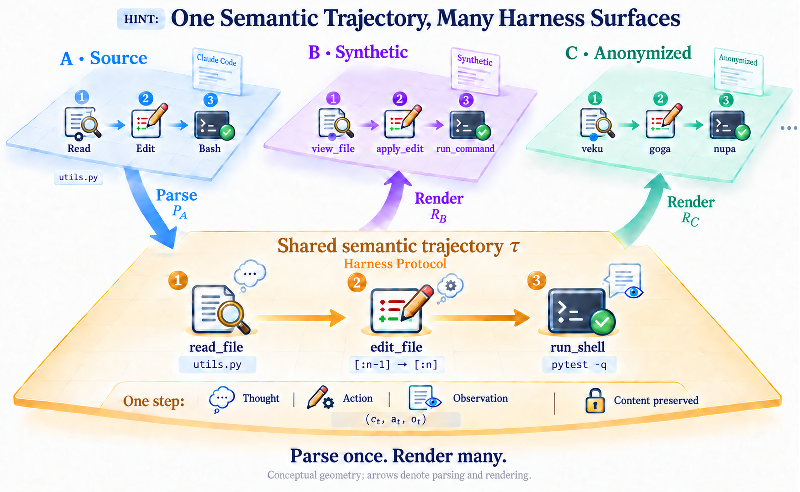
\includegraphics[width=\textwidth]{pic/intro_hint_protocol_geometry_v4.pdf}
\end{center}
\caption{One protocol trajectory and three of its surfaces. Parsing the source
trajectory ($P_A$) yields $\tau = [(c_t, a_t, o_t)]$; rendering it under two
other configurations, one with synthetic tool names ($R_B$) and one with
anonymized identifiers ($R_C$), produces counterfactual harnesses that never
existed but carry the same episode. Proposition~1 states that every such
surface parses back to the same $\tau$: the content of the episode is
preserved and only the surface changes.}
\label{fig:orbit}
\end{figure}

\section{Behavioural analysis of the evaluation trajectories}
\label{app:analysis}

Accuracy summarizes an episode in one bit. The trajectories behind this
paper's cross-harness evaluations carry more: every tool call, the observation
it produced, the tokens each step consumed, and how the episode ended. This
appendix reads them. Two collections are used. The first is a models $\times$
harnesses evaluation: six instruction-tuned models (Claude Opus 5, GPT-5.6,
DeepSeek-V4-Pro, GLM-5.2, \basemodel{}, Qwen3.5-27B) run under the four
production harnesses and \cham{} (one fixed synthetic configuration) on the
$500$ Verified and $300$ Multilingual tasks (Qwen3.5-27B on a $100+60$
subset), $17{,}374$ completed episodes over $26$ model--harness cells, of which
$17{,}230$ made at least one tool call and enter Table~\ref{tab:ana-summary};
Figure~\ref{fig:ana-mix} marks the cells that could not be run. The second is
the \method{} and control pair of the earlier \oldmodel{} run
(Appendix~\ref{app:e1-30b}), on \claudecode{} (the source harness),
\opencode{} and \openhands{}: $4{,}280$
episodes. Every call is mapped to the protocol vocabulary with the parsers of
Section~\ref{sec:protocol}, and shell commands are further labelled by intent
(read, search, edit, run tests, other), so that a \texttt{sed -n} issued in
\codexcli{} and a \texttt{Read} issued in \claudecode{} count as the same
thing. Episodes that ended in an infrastructure exception are excluded from
behavioural statistics, and one cell, Claude Opus 5 $\times$ \codexcli{}, is
dropped entirely: $57\%$ of its episodes were cut short by an API-gateway
error after two or three calls. The frontier models were reached through a
gateway, so this appendix draws no conclusion from the absolute accuracy of
any single API cell; the behavioural quantities below are robust to that.

\begin{figure}[t]
\begin{center}
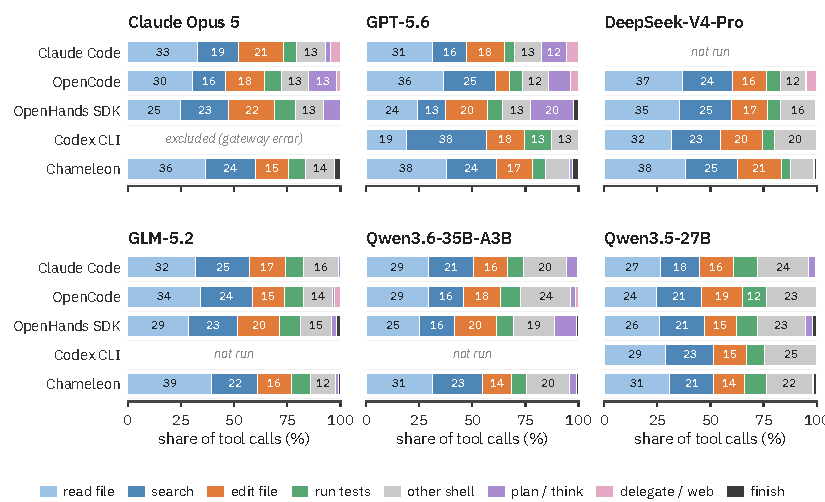
\includegraphics[width=\textwidth]{pic/ana_action_mix.pdf}
\end{center}
\caption{The same model does the same semantic work in every harness. Each
row is one model--harness cell; segments are the share of the cell's tool
calls that read a file, search, edit, run tests, run other shell commands,
plan or think, delegate or fetch the web, or finish, after normalization to
the protocol vocabulary and intent-labelling of shell commands. Numbers are
percentages; rows within a panel differ from one another about as much as the
same row differs across panels.}
\label{fig:ana-mix}
\end{figure}

\subsection{Semantic action composition}

Figure~\ref{fig:ana-mix} gives, for each model and harness, the mix of
semantic actions after normalization. The rows within a panel are strikingly
alike. Moving a model between harnesses shifts its action mix by a median
Jensen--Shannon divergence of $0.025$ bits; moving between models under a
fixed harness shifts it by $0.027$ bits. The harness, in other words, changes
what a model does about as little as the choice of model does, and both
changes are small. What does move is exactly what the harness makes explicit:
planning calls exist only where a harness declares a task tracker
(\texttt{TodoWrite} in \claudecode{}, \texttt{todowrite} in \opencode{},
\texttt{task\_tracker} in \openhands{}), and a terminating call only where the harness requires one
(\openhands{}, \cham{}). \codexcli{} is the one surface that visibly reshapes
behaviour: with no first-class search tool, GPT-5.6 spends $38\%$ of its calls
searching there against $13$--$25\%$ elsewhere, the exploration that a single
\texttt{Grep} or \texttt{Glob} delivers in other harnesses being spread over
several shell invocations.

\begin{figure}[t]
\begin{center}
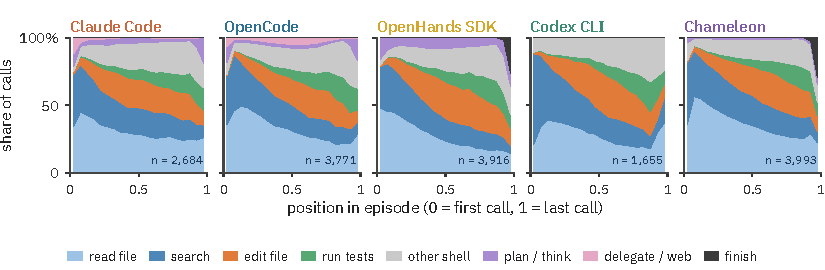
\includegraphics[width=\textwidth]{pic/ana_phase.pdf}
\end{center}
\caption{Where in an episode each kind of call happens, pooled over the six
models (episodes with at least ten calls, $n$ per panel). Every harness shows
the same arc from exploration to editing to testing; harness conventions sit
at the two ends, planning and delegation at the start where a harness offers
them, an explicit finish at the end where a harness requires one.}
\label{fig:ana-phase}
\end{figure}

Figure~\ref{fig:ana-phase} resolves the same calls over the course of an
episode. Every harness shows one arc: reads and searches make up $70$--$90\%$
of the first calls, editing grows through the middle, and testing rises toward
the end. Conventions occupy the two ends. \claudecode{} and \opencode{} open
with planning and delegation calls ($21\%$ and $18\%$ of the calls in the
opening $5\%$ of an episode), \openhands{} and \cham{} close with an
explicit finish ($26\%$ and $30\%$ of the calls in the closing $5\%$), and
\codexcli{} opens with a search-dominated burst ($67\%$ of its opening
calls). Below the conventions, the coarse action composition is the same.

\subsection{Episode length and context cost}

\begin{figure}[t]
\begin{center}
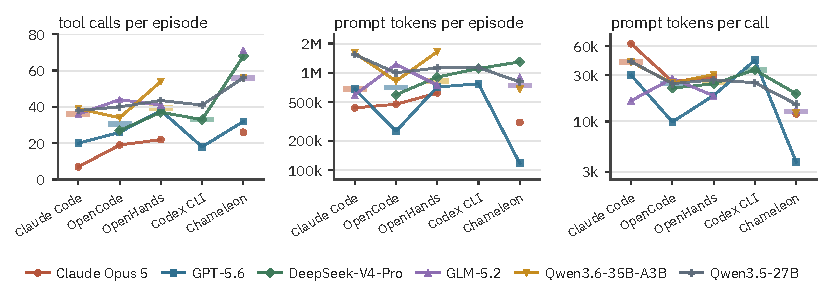
\includegraphics[width=\textwidth]{pic/ana_episode_cost.pdf}
\end{center}
\caption{Episode length and context cost by harness. Per model (lines) and
pooled over models (short bars): the median number of tool calls per episode,
the median prompt tokens summed over an episode, and the median prompt tokens
per call, a proxy for the context the model reads at each step. The same
semantic work costs up to $3.4\times$ more tokens per call depending only on
the surface.}
\label{fig:ana-cost}
\end{figure}

\begin{table}[t]
\caption{Per-harness summary, pooled over the six models (episodes with at
least one call; \codexcli{} covers the three models that could be run under
it). Tokens per call is the median over episodes of prompt tokens divided by
calls. ``Rejected'' counts calls the harness refused before executing them,
per $100$ calls; ``edit miss'' is the share of edit calls whose anchor text was
not found in the file.}
\label{tab:ana-summary}
\begin{center}
\begin{small}
\begin{tabular}{lrrrrrrr}
\toprule
Harness & Episodes & Calls & Prompt tok. & Tok./call & Reads & Rejected & Edit miss \\
\midrule
\claudecode{}  & $3{,}304$ & $22$ & $741$k & $38.4$k & $31\%$ & $0.27$ & $5.0\%$ \\
\opencode{}    & $4{,}084$ & $29$ & $569$k & $22.0$k & $33\%$ & $0.10$ & $1.9\%$ \\
\openhands{}   & $4{,}064$ & $37$ & $864$k & $24.4$k & $28\%$ & $0.99$ & $0.6\%$ \\
\codexcli{}    & $1{,}747$ & $23$ & $925$k & $36.9$k & $28\%$ & $0.11$ & $0.4\%$ \\
\cham{}        & $4{,}031$ & $46$ & $487$k & $11.2$k & $36\%$ & $0.41$ & $1.6\%$ \\
\bottomrule
\end{tabular}
\end{small}
\end{center}
\end{table}

If the harness leaves the semantic policy alone, what does it change?
Figure~\ref{fig:ana-cost} and Table~\ref{tab:ana-summary} answer: how much the
same work costs. Pooled over models, the median episode takes $22$ calls in
\claudecode{} and $46$ in \cham{}, and the median prompt tokens per call
range from $11$k in \cham{} to $38$k in \claudecode{}, a $3.4\times$
difference for the same semantic actions. The per-call cost is set by the
surface: the system prompt and tool documentation a harness prepends, the
verbosity of its observations, and whether it compacts context.
\claudecode{}'s $21$-tool schema and \codexcli{}'s shell-only surface, whose
observations are raw command output, are the most expensive per call;
\cham{}'s terse documentation and $2{,}000$-character observation cap are the
cheapest. The two quantities can move in opposite directions: \cham{} takes
the most calls but the fewest tokens per call, and its total episode cost is
the lowest of all harnesses for four of the six models.

\subsection{Task-level agreement across harnesses}

\begin{figure}[t]
\begin{center}
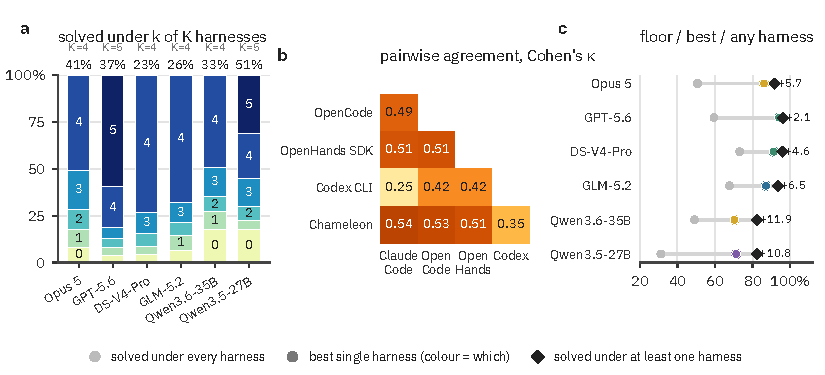
\includegraphics[width=\textwidth]{pic/ana_agreement.pdf}
\end{center}
\caption{Task-level agreement across harnesses, per model, over tasks with a
settled outcome under every harness the model was run in ($K$ harnesses).
(a)~Share of tasks solved under exactly $k$ of the $K$ harnesses; the number
above each bar is the harness-dependent share, $0<k<K$. (b)~Pairwise Cohen's
$\kappa$ between the sets of tasks two harnesses solve, averaged over the
models that were run under both. (c)~Per model: tasks solved under every
harness, under the best single harness (coloured by which), and under at
least one; the label is the gap between the last two, in points.}
\label{fig:ana-agree}
\end{figure}

A headline table reports one accuracy per harness; Figure~\ref{fig:ana-agree}
asks whether the harnesses solve the \emph{same} tasks. They do not. Between
$23\%$ (DeepSeek-V4-Pro) and $51\%$ (Qwen3.5-27B) of a model's tasks are
harness-dependent, solved under some harnesses and not others
(Figure~\ref{fig:ana-agree}a), and the agreement between any two harnesses on
which tasks a model solves is only moderate, Cohen's $\kappa$ between $0.25$
and $0.54$ (Figure~\ref{fig:ana-agree}b); \codexcli{} agrees least with the
rest. Consequently an oracle that may pick the harness per task beats the best
single harness by $2.1$ (GPT-5.6) to $11.9$ (\basemodel{}) points
(Figure~\ref{fig:ana-agree}c), and the gap widens as the model weakens. Part of
this gap is the run-to-run variance a single harness would also show
($\pm2.0$ points, Appendix~\ref{app:eval}); the remainder is what the interface,
not the task, decided. Two readings follow. The spread of a headline table
understates interface dependence, since accuracies can agree while the solved
sets do not; and the oracle gap bounds what a policy that is indifferent to
the interface could recover.

\subsection{Interface errors}

\begin{figure}[t]
\begin{center}
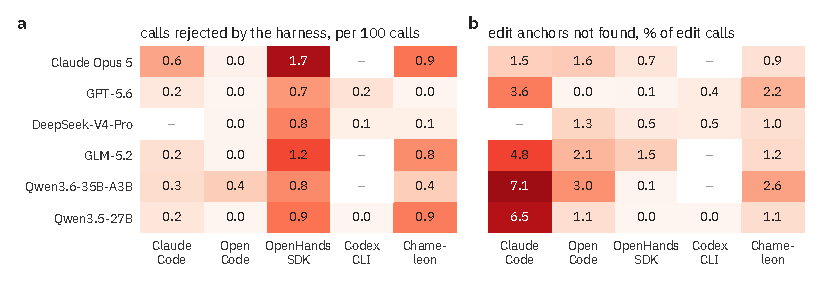
\includegraphics[width=\textwidth]{pic/ana_interface_errors.pdf}
\end{center}
\caption{Harness-reported interface errors by model and harness.
(a)~Calls the harness refused before executing them: a tool that does not
exist, malformed arguments, or a violated convention, per $100$ calls.
(b)~Edit calls whose anchor text was not found in the file, as a share of edit
calls. Both read down the columns: which harness a model is in predicts its
friction better than which model it is.}
\label{fig:ana-friction}
\end{figure}

Harnesses also differ in how often they refuse what the model says.
Figure~\ref{fig:ana-friction} counts two classes of harness-reported error.
Calls rejected before execution (Figure~\ref{fig:ana-friction}a) are rare
everywhere except \openhands{}, where every model has its highest rate
($0.7$--$1.7$ per $100$ calls). Of those rejections, $1{,}831$ across the six
models carry the same message, ``Cannot execute multiple commands at once'', a
convention no other harness has and every model violates. Edit calls whose
anchor text is not found (Figure~\ref{fig:ana-friction}b) are highest under
\claudecode{} for every model ($1.5$--$7.1\%$ of edits) and near zero under
\openhands{} for the same models ($\le 1.5\%$): \claudecode{}'s \texttt{Edit}
enforces a stricter contract than the others: a unique anchor ($504$ refusals
for a missing and $82$ for an ambiguous one, over all models), a change that
is not empty ($257$), and, counted in panel~(a), a read of the file before it
is edited ($166$). Both panels
read down the columns rather than across the rows. Friction follows the interface more than the model, and it is exactly the kind of property a surface-bound policy
learns to avoid in one harness and then runs into in the next.

\subsection{\method{} and the control off the source harness}

\begin{figure}[t]
\begin{center}
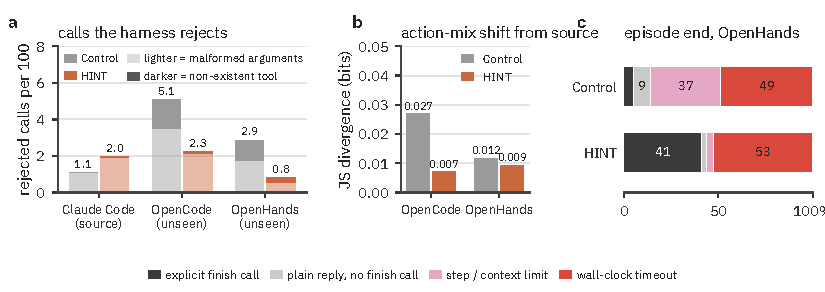
\includegraphics[width=\textwidth]{pic/ana_hint_behaviour.pdf}
\end{center}
\caption{Interface behaviour of \method{} and the \control{} on the source
harness and on two unseen ones (trajectories of the earlier run,
Appendix~\ref{app:e1-30b}). (a)~Calls the harness
refused, per $100$ calls, split into malformed arguments and calls to a tool
that does not exist. (b)~Jensen--Shannon divergence between a model's semantic
action mix on an unseen harness and its own mix on the source harness.
(c)~How episodes end on \openhands{}, whose convention is an explicit finish
call; both arms hit the wall clock often, which is why no \openhands{} accuracy
enters a conclusion (Appendix~\ref{app:e1-30b}), but among the episodes that do
not, \method{} follows the convention and the control does not.}
\label{fig:ana-hint}
\end{figure}

Appendix~\ref{app:e1-30b} compares that run's two models by accuracy. Their
trajectories show what the accuracy is made of. On the source harness the two
arms are alike: $1.1$ and $2.0$ rejected calls per $100$
(Figure~\ref{fig:ana-hint}a), the same action mix, the same edit precision
($24\%$ and $22\%$ of edits miss their anchor). Off the source harness they
diverge. On \opencode{} the control's rejection rate rises to $5.1$ per $100$
calls, $1.6$ of them calls to tools that do not exist, with names that belong
to no harness (\texttt{bshell}, \texttt{browsetree}, \texttt{bqrtask});
\method{}'s stays at $2.3$ with $0.1$ non-existent tools. On \openhands{} the
rates are $2.9$ against $0.8$. The control also reads paths that do not exist
six times as often on \opencode{} as \method{} does ($7.2$ against $1.2$ per
$100$ calls; $0.14$ and $0.22$ on the source harness), and its edits miss
their anchor more often ($32\%$ against $19\%$). Its semantic action mix
moves away from its own source-harness behaviour by $0.027$ bits on
\opencode{} where \method{}'s moves by $0.007$ (Figure~\ref{fig:ana-hint}b).
The clearest signal is the completion convention
(Figure~\ref{fig:ana-hint}c). \openhands{} expects an explicit finish call;
\claudecode{}, the source harness, expects a plain reply. Among episodes that
did not hit the wall clock, \method{} ends with the finish call $87\%$ of the
time and the control $10\%$, the control instead stopping with a plain reply
or running into the step limit, that is, carrying the source harness's
convention into a harness that does not have it. Even on the source harness,
the control runs into the four-hour wall clock in $53\%$ of episodes against
$36\%$ for \method{}. These are the behaviours the accuracy in
Table~\ref{tab:e1-30b} averages over, and they are what interface invariance
means at the level of a single call.

\begin{figure}[t]
\begin{footnotesize}
\begin{verbatim}
(1) Control on OpenHands SDK: the file editor called with the
    argument schema of Claude Code's Bash tool
    call     str_replace_editor
             {"command": "grep -n \"def write\\|class Basic\"
                          /testbed/astropy/io/ascii/basic.py | head -30",
              "description": ""}
    harness  ERROR: flag provided but not defined: -description

(2) Control on OpenCode: a tool that no harness declares
    call     bshell {...}
    harness  Model tried to call unavailable tool 'bshell'.
             Available tools: bash, edit, glob, grep, invalid, read,
             skill, task, todowrite, webfetch, write.

(3) Qwen3.5-27B on Codex CLI: a memorized call template emitted as
    text on the second turn, after one structured call to `shell`
    model    user
             <tool_call>
             <function=exec_command>
             <parameter=cmd>
             find /testbed -type f -name "python.py" | grep domain
             </parameter>
             </function>
             </tool_call>
    harness  (no call parsed; the text is taken as the final answer
             and the episode ends)
\end{verbatim}
\end{footnotesize}
\caption{Three interface failures, verbatim. (1)~The control applies the
argument schema of its source harness's shell tool (\texttt{command} plus
\texttt{description}) to a different harness's file editor
(\texttt{str\_replace\_editor}, the editor of the \openhands{} build used in
that run; Appendix~\ref{app:eval}). (2)~It names a tool that exists nowhere. (3)~An instruction-tuned model, after one correct
structured call, falls back to a call template it memorized, naming
\texttt{exec\_command}, the shell entry point of the \codexcli{} release in
our parsed corpus (Table~\ref{tab:harnesses}), inside its own text markup;
the release under evaluation exposes the shell as \texttt{shell} and accepts
only structured calls, so the episode ends. $47$ of Qwen3.5-27B's $81$ failed
\codexcli{} episodes end this way.}
\label{fig:ana-examples}
\end{figure}

Figure~\ref{fig:ana-examples} shows three of these failures verbatim. The
first two are the control's: it calls \openhands{}'s file editor with the
argument schema of \claudecode{}'s \texttt{Bash} tool, and it calls tools that
exist nowhere. The third is not from a fine-tuned model but from an instruction-tuned
model in the models $\times$ harnesses evaluation, and it is the purest form
of interface reliance we observed: after one correct structured call, the
model emits, as text, a call template it learned somewhere else, with a tool
name from a different release of the same harness. The harness in front of it
has told it, in the system prompt, what its tools are called and how to call
them; the memorized surface wins anyway. $47$ of the model's $81$ failed
\codexcli{} episodes end on such a line, after a median of one call. This is
the failure that \method{} is designed to remove, and the reason the
anonymized tier of Section~\ref{sec:method} exists: a model that has learned
to read the tool documentation in front of it has nothing to fall back on.

\section{An earlier run on \oldmodel{}}
\label{app:e1-30b}

Before the experiment of Section~\ref{sec:step-matched} we ran the same comparison at a
smaller scale on \oldmodel{} \citep{qwen3,qwen3_30b_card}, with a different
recipe on both sides. The data were $5{,}000$ \claudecode{} trajectories;
\chr{} rendered the $4{,}133$ of them that passed the filters of Section~\ref{sec:setup} into $M=2$ surfaces each, giving $8{,}266$ samples under
$8{,}204$ distinct surface configurations with $11{,}205$ distinct tool names.
\method{} trained on all $5{,}000$ real trajectories \emph{mixed with} the
$8{,}266$ renderings ($13{,}266$ samples) and the control on the real
trajectories alone, each for the same number of optimizer steps at a global
batch of $32$ and learning rate $5\times10^{-5}$; for the control this is about $6.2$
passes over its data. Matching sample counts instead would have given the
control $27\%$ more tokens, since the rendered samples are $34\%$ shorter than
the originals. Each cell was evaluated once, through a different serving endpoint from
Section~\ref{sec:setup}.

\begin{table}[t]
\caption{The earlier run: pass@1 (\%), one evaluation per cell. Base is the
model before fine-tuning, under the same harness; $\Delta$ is \method{} minus
control, and bold marks the better of the two.}
\label{tab:e1-30b}
\begin{center}
\begin{small}
\setlength{\tabcolsep}{4.5pt}
\begin{tabular}{@{}l S[table-format=2.1] S[table-format=2.1] S[table-format=2.1] S[table-format=+1.1] @{\hspace{16pt}} S[table-format=2.1] S[table-format=2.1] S[table-format=2.1] S[table-format=+1.1]@{}}
\toprule
 & \multicolumn{4}{c}{\swev{}} & \multicolumn{4}{c}{\swem{}} \\
\cmidrule(r){2-5}\cmidrule(l){6-9}
Harness & {Base} & {Control} & {\method{}} & {$\Delta$} & {Base} & {Control} & {\method{}} & {$\Delta$} \\
\midrule
\claudecode{} (source) & 25.2 & 47.8 & \bfseries 48.2 & +0.4 & 14.7 & 33.7 & \bfseries 35.7 & +2.0 \\
\opencode{}            & 16.0 & \bfseries 43.0 & 42.0 & -1.0 & 13.3 & 23.3 & \bfseries 31.0 & +7.7 \\
\bottomrule
\end{tabular}
\end{small}
\end{center}
\end{table}

Table~\ref{tab:e1-30b} gives the result. Two differences exceed the noise
floor, both on Multilingual: $2.0$ points on \claudecode{} and $7.7$ points in
the unseen-harness cell, \opencode{} ($93/300$ against $70/300$). Measured as the accuracy each model loses
when moved from \claudecode{} to \opencode{}, \method{} loses $4.7$ points on
Multilingual against the control's $10.3$, but $6.2$ on Verified against the control's
$4.8$: on Verified this run shows no benefit. The \openhands{} runs of this
comparison are not reported: both models timed out at high rates ($25\%$ and $64\%$ of settled
trials), traced to a proactive-compaction threshold set above the context
length actually reached, so that per-step prefill grew until the wall clock ran
out. Appendix~\ref{app:analysis} uses this run's trajectories, \openhands{}
included, only for statistics that do not depend on accuracy.

\section{Evaluation details}
\label{app:eval}

\paragraph{Rounding.} Pass rates are pass counts over task counts, shown to
one decimal. Spreads and the differences quoted in the text are computed from
the counts for single-evaluation cells and from the per-cell means shown for
the three-evaluation cells of Table~\ref{tab:e1}, then rounded once, so they
can differ from the difference of two displayed values by $0.1$.

\paragraph{Noise floor.} Two submissions of one configuration, the \method{}
model of Appendix~\ref{app:e1-30b} under \openhands{} in the conditions of
that appendix, differed by $2.0$ points on the $500$-task set ($52.0\%$ and
$54.0\%$) and by $1.0$ point on the $300$-task set ($34.3\%$ and $33.3\%$). We
use these differences as the single-evaluation noise floor for every cell,
$\pm2.0$ on Verified and $\pm1.0$ on Multilingual, and do not interpret
differences below them. The floor rests on one repeated pair and is a reading
rule rather than a variance estimate.

\paragraph{Harness releases.} The releases evaluated here are \claudecode{}
2.1.140, \codexcli{} 0.142.0, \opencode{} 1.17.15 and \openhands{} 1.40.1.
They differ from those of the parsed corpora (Table~\ref{tab:harnesses}) in a
few tool names:
\codexcli{} exposes its shell as \texttt{shell} rather than
\texttt{exec\_command}, and the \openhands{} build used for the earlier run
(Appendix~\ref{app:e1-30b}) exposes \texttt{execute\_bash} and
\texttt{str\_replace\_editor} in place of \texttt{terminal} and
\texttt{file\_editor} and has no task tracker. Figure~\ref{fig:ana-examples}
quotes the evaluated names verbatim.

\paragraph{Settings of every experiment.} Table~\ref{tab:settings} lists, for
each experiment, the models compared, the harnesses and benchmarks, the number
of evaluations per cell, and whether the runs share the serving stack of
Section~\ref{sec:setup}.

\begin{table}[ht]
\caption{Settings of every experiment. ``Section~\ref{sec:setup} stack'' is the
vLLM serving stack of Section~\ref{sec:setup}; ``Appendix~\ref{app:e1-30b}
conditions'' is the earlier serving endpoint.}
\label{tab:settings}
\begin{center}
\begin{footnotesize}
\setlength{\tabcolsep}{2.5pt}
\newcolumntype{L}[1]{>{\raggedright\arraybackslash}p{#1}}
\begin{tabular}{@{}L{0.68in}L{0.9in}L{1.05in}L{0.85in}L{0.36in}L{0.27in}L{0.94in}@{}}
\toprule
Where & Base model & Models compared & Harnesses & Bench. & Evals & Conditions \\
\midrule
Section~\ref{sec:harness-choice}, Table~\ref{tab:e0} & Qwen3.5-35B-A3B, \basemodel{}, KAT-Coder-V2.5-Dev & not fine-tuned & four production, \cham{} & V, M & 1 & Section~\ref{sec:setup} stack \\
Section~\ref{sec:step-matched}, Table~\ref{tab:e1} & \basemodel{} & \method{}, \control{} & four production, \cham{} & V, M & 3 & Section~\ref{sec:setup} stack \\
Section~\ref{sec:real}, Figure~\ref{fig:real} & \oldmodel{} & \method{} of Appendix~\ref{app:e1-30b}, real-trajectory model & four production, \cham{} & V, M & 1 & Appendix~\ref{app:e1-30b} conditions for \claudecode{} and \opencode{}, separate runs elsewhere \\
Section~\ref{sec:anon}, Figure~\ref{fig:anon} & \basemodel{} & base, \method{} of Table~\ref{tab:e1} & \cham{}, three naming settings & M & 1 & separate runs \\
Section~\ref{sec:axes}, Figure~\ref{fig:axes} & \oldmodel{} & \method{} of Appendix~\ref{app:e1-30b}, control & \cham{}, seven surfaces & M & 1 & separate runs; unfinished episodes excluded \\
Appendix~\ref{app:e1-30b}, Table~\ref{tab:e1-30b} & \oldmodel{} & \method{}, control & \claudecode{}, \opencode{} & V, M & 1 & Appendix~\ref{app:e1-30b} conditions \\
\bottomrule
\end{tabular}
\end{footnotesize}
\end{center}
\end{table}

\end{document}
